
\chapter{Data collection and processing}
\label{chap:methods}

% NC: In general here be careful not to go overboard with details. I've tried to make it a bit more concise. We don't want your poor examiner to expire with the weight of the thesis esp as it's already 40 pages without the main chapter!!!
	%I've cut it down and created a new appendix at the end
\section{Overview}

	I compiled a morphological data set of both photographs and linear measurements from 366 specimens representing 99 species of small mammals. 
	%(total number of skulls and species in Access Data base, excluding the two _sp.)
	I collected morphological data from skulls, limbs and skins. I have divided my description of how the data were collected and processed into three sections:
	
	\begin{enumerate}[i]
	
	\item Data collection (section \ref{sect:datacollection}): \\
	Summary of the species measured, taxonomic identification,  photographic set up and image processing.
	
	\item Geometric morphometric analyses (section \ref{sect:morphometrics}):\\
	Landmark and semilandmark placement on different views of skulls and mandibles.
	
	
	\item Additional data collection (appendix \ref{appendix}) \\
	In this thesis I only analysed a subset of the total data that I collected. Therefore, the additional data represent a significant resource for future work. I have documented collection of these data (linear measurements of skulls and limbs and photographs of skins) in appendix \ref{appendix} at the end of my thesis.
	%Maybe take out the references to skins?
	
	\end{enumerate} 


%####################################################
\section{Data collection}
\label{sect:datacollection}
%##################################################


\subsection{\normalfont{Species measured and taxonomy}}

	Between January and September 2013, I spent a total of 9 weeks working in the collections of five museums: the Natural History Museum, London (BMNH), the Smithsonian Institute Natural History Museum, Washington D.C. (SI), the American Museum of Natural History, New York (AMNH), Museum of Comparative Zoology, Cambridge M.A. (MCZ) and the Field Museum of Natural History, Chicago (FMNH). I measured and photographed 366 skulls, 248 post-cranial skeletons and 277 skins from 101 species belonging to seven Families within four Orders: Afrosoricida (Tenrecidae, Chrysochloridae), Erinaceomorpha (Erinaceidae), Soricomorpha (Soricidae, Solenodontidae, Talpidae) and Notoryctemorphia (Notoryctidae). 

	I measured all the tenrecs and golden moles available in the collections (31 species of tenrec, 12 species of golden moles out of 34 and 21 species in each Family respectively, table \ref{tab:species.measured}). 
	For my comparative species of non-Afrosoricida species, I chose a random sample of 56 taxa which have been previously identified as convergent with tenrecs \citep[e.g.][]{Gould1966, Symonds2005, Poux2008, Olson2013}. I only analysed the Afrosoricida species for this thesis, details about the additional taxa can be found in appendix \ref{appendix}.
	
	I recorded species names as they were written on museum specimen labels and then corrected them to match the taxonomy in Wilson and Reeder's Mammal Species of the World \citeyearpar{Wilson2005}. For recently identified species,  which are not included in Wilson and Reeder \citeyearpar{Wilson2005} I used the taxonomy recorded on the specimen labels.

	Wilson and Reader \citeyearpar{Wilson2005} record 30 species of tenrec but more recent studies indicate that there are now 34 species\citep[][Table \ref{tab:species.measured}]{Olson2013}. The additional species belong to the shrew tenrec (\textit{Microgale}) Genus and represent either recognition of cryptic species boundaries \citep{Olson2004} or discovery of new species \citep{Goodman2006, Olson2009}. Only one of these four recent additions, \textit{M. jobihely}, was present in the museum collections and therefore I could not include the three other newly recognised species in my analyses.

	Table \ref{tab:species.measured} outlines the number of species I measured from each Family and how this sample relates to the overall number of species in that Family.

%------------------------------------------------
%Species.measured table

%I added the %coverage, still need to figure out spacing for the centred columns

\begin{table}[h]
	\caption[Species measured] 
	{The number of species measured in each Family compared to the total number of species in that Family (coverage is the percentage of species from each Family that are represented in my data). The total number of species in each family is according to Mammal Species of the World version 3 \citep{Wilson2005} with the exception of the Tenrecidae: there are now 34 identified species compared to 30 recognised in Wilson and Reeder (\citeyear{Wilson2005}).}
	%Species.measured table
%To get the number measured for each Family, I counted the number of unique species in my Tb_Taxonomy Access table for that family
%So it's the number of species measured overall but that doesn't necessarily mean that I have the same number in every data set
%I didn't count the _sp. specimens as separate species

%I took out the reference to the IUCN because it seems to only list species that are threatened/endangered rather than a full list of all species in a family

\begin{tabular}{p{3.4cm}p{3cm}p{2cm}p{2cm}p{2cm}}

\hline
\textbf{Order} & \textbf{Family} & \textbf{Measured species} & \textbf{Total species} & \textbf{Coverage} \\
\hline
%----------------------------------------------------
Afrosoricida & Tenrecidae & 31 & 34 & 91 \% \\
%-------------------------------------------------
Afrosoricida & Chrysochloridae & 12 & 21 & 57 \% \\
%----------------------------------------------------
Erinaceomorpha & Erinaceidae & 16 & 24 & 67 \% \\
%----------------------------------------------------
Soricomorpha & Soricidae & 22 & 376 & 5.8 \% \\
%----------------------------------------------------
Soricomorpha & Solenodontidae & 2 & 4 & 50 \% \\
%----------------------------------------------------
Soricomorpha & Talpidae & 15 & 39 & 38 \% \\
%----------------------------------------------------
Notoryctemorphia & Notoryctidae & 1 & 2 & 50 \% \\
%-----------------------------------------------
\hline

\end{tabular}

%*There are now 34 recognised tenrec species \citep{Olson2013}	
	\label{tab:species.measured}
\end{table}
 
%-----------------------------------------#

	%Moved this paragraph up from the error checking
	I included both male and female specimens in my data as I am interested in cranial shape of the species as a whole regardless of whether or not there are differences due to sexual size dimorphism. Age classification of mammal skulls is usually based on dental characteristics and cranial fusion but it is difficult to classify tenrecs in this way. In some species the last molar does not erupt fully until the first molar has been shed so the full dentition is never present at any one time \citep{Nowak1983}. Furthermore, it is difficult to distinguish deciduous from permanent teeth in \textit{Microgale} tenrecs \citep{Asher2008} which has led to confusion and misidentification of juvenile forms as separate species \citep{Olson2004}.
	Therefore, I identified and excluded any obviously juvenile specimens based on incomplete cranial fusion. When specimens could not be obviously identified as juveniles I treated them all as equivalent adult forms. 	



%------------------------------------------------
%Moved the specimen labels and linear measurements into the appendix
%-----------------------------------------
\subsection{\normalfont{Photographing specimens}}

	In order to get 2D landmarks for my specimens, I first had to photograph them. I used photographic copy stands consisting of a camera attachment with an adjustable height bar, a flat stage on which to place the specimen and an adjustable light source. To take possible light variability into account, on each day I took a photograph of a white sheet of paper and used the custom white balance function on the camera to set the image as the baseline "white" measurement for those particular light conditions.
	
	I photographed the specimens with a Canon EOS 650D camera fitted with a EF 100 mm f/2.8 Macro USM lens. I used a remote control (H\"ahnel Combi TF) to take the photos to avoid shaking the camera and distorting the images. I photographed the specimens on a black material background. I placed the light source from the top left-hand corner of the photograph and positioned a piece of white card on the bottom right side of the specimen which reflected the light back onto the specimen and minimised any shadows (figure \ref{fig:camera}). I used small bean bags as necessary to hold the specimens in position while being photographed to ensure that the specimen lay in a flat plane relative to the camera and did not tilt in any direction. I used the grid-line function on the live-view display screen of the camera to position the specimens in the centre of each image. 

%----------------------------------------------
%Camera picture
\begin{figure}[h] 
  \centering
  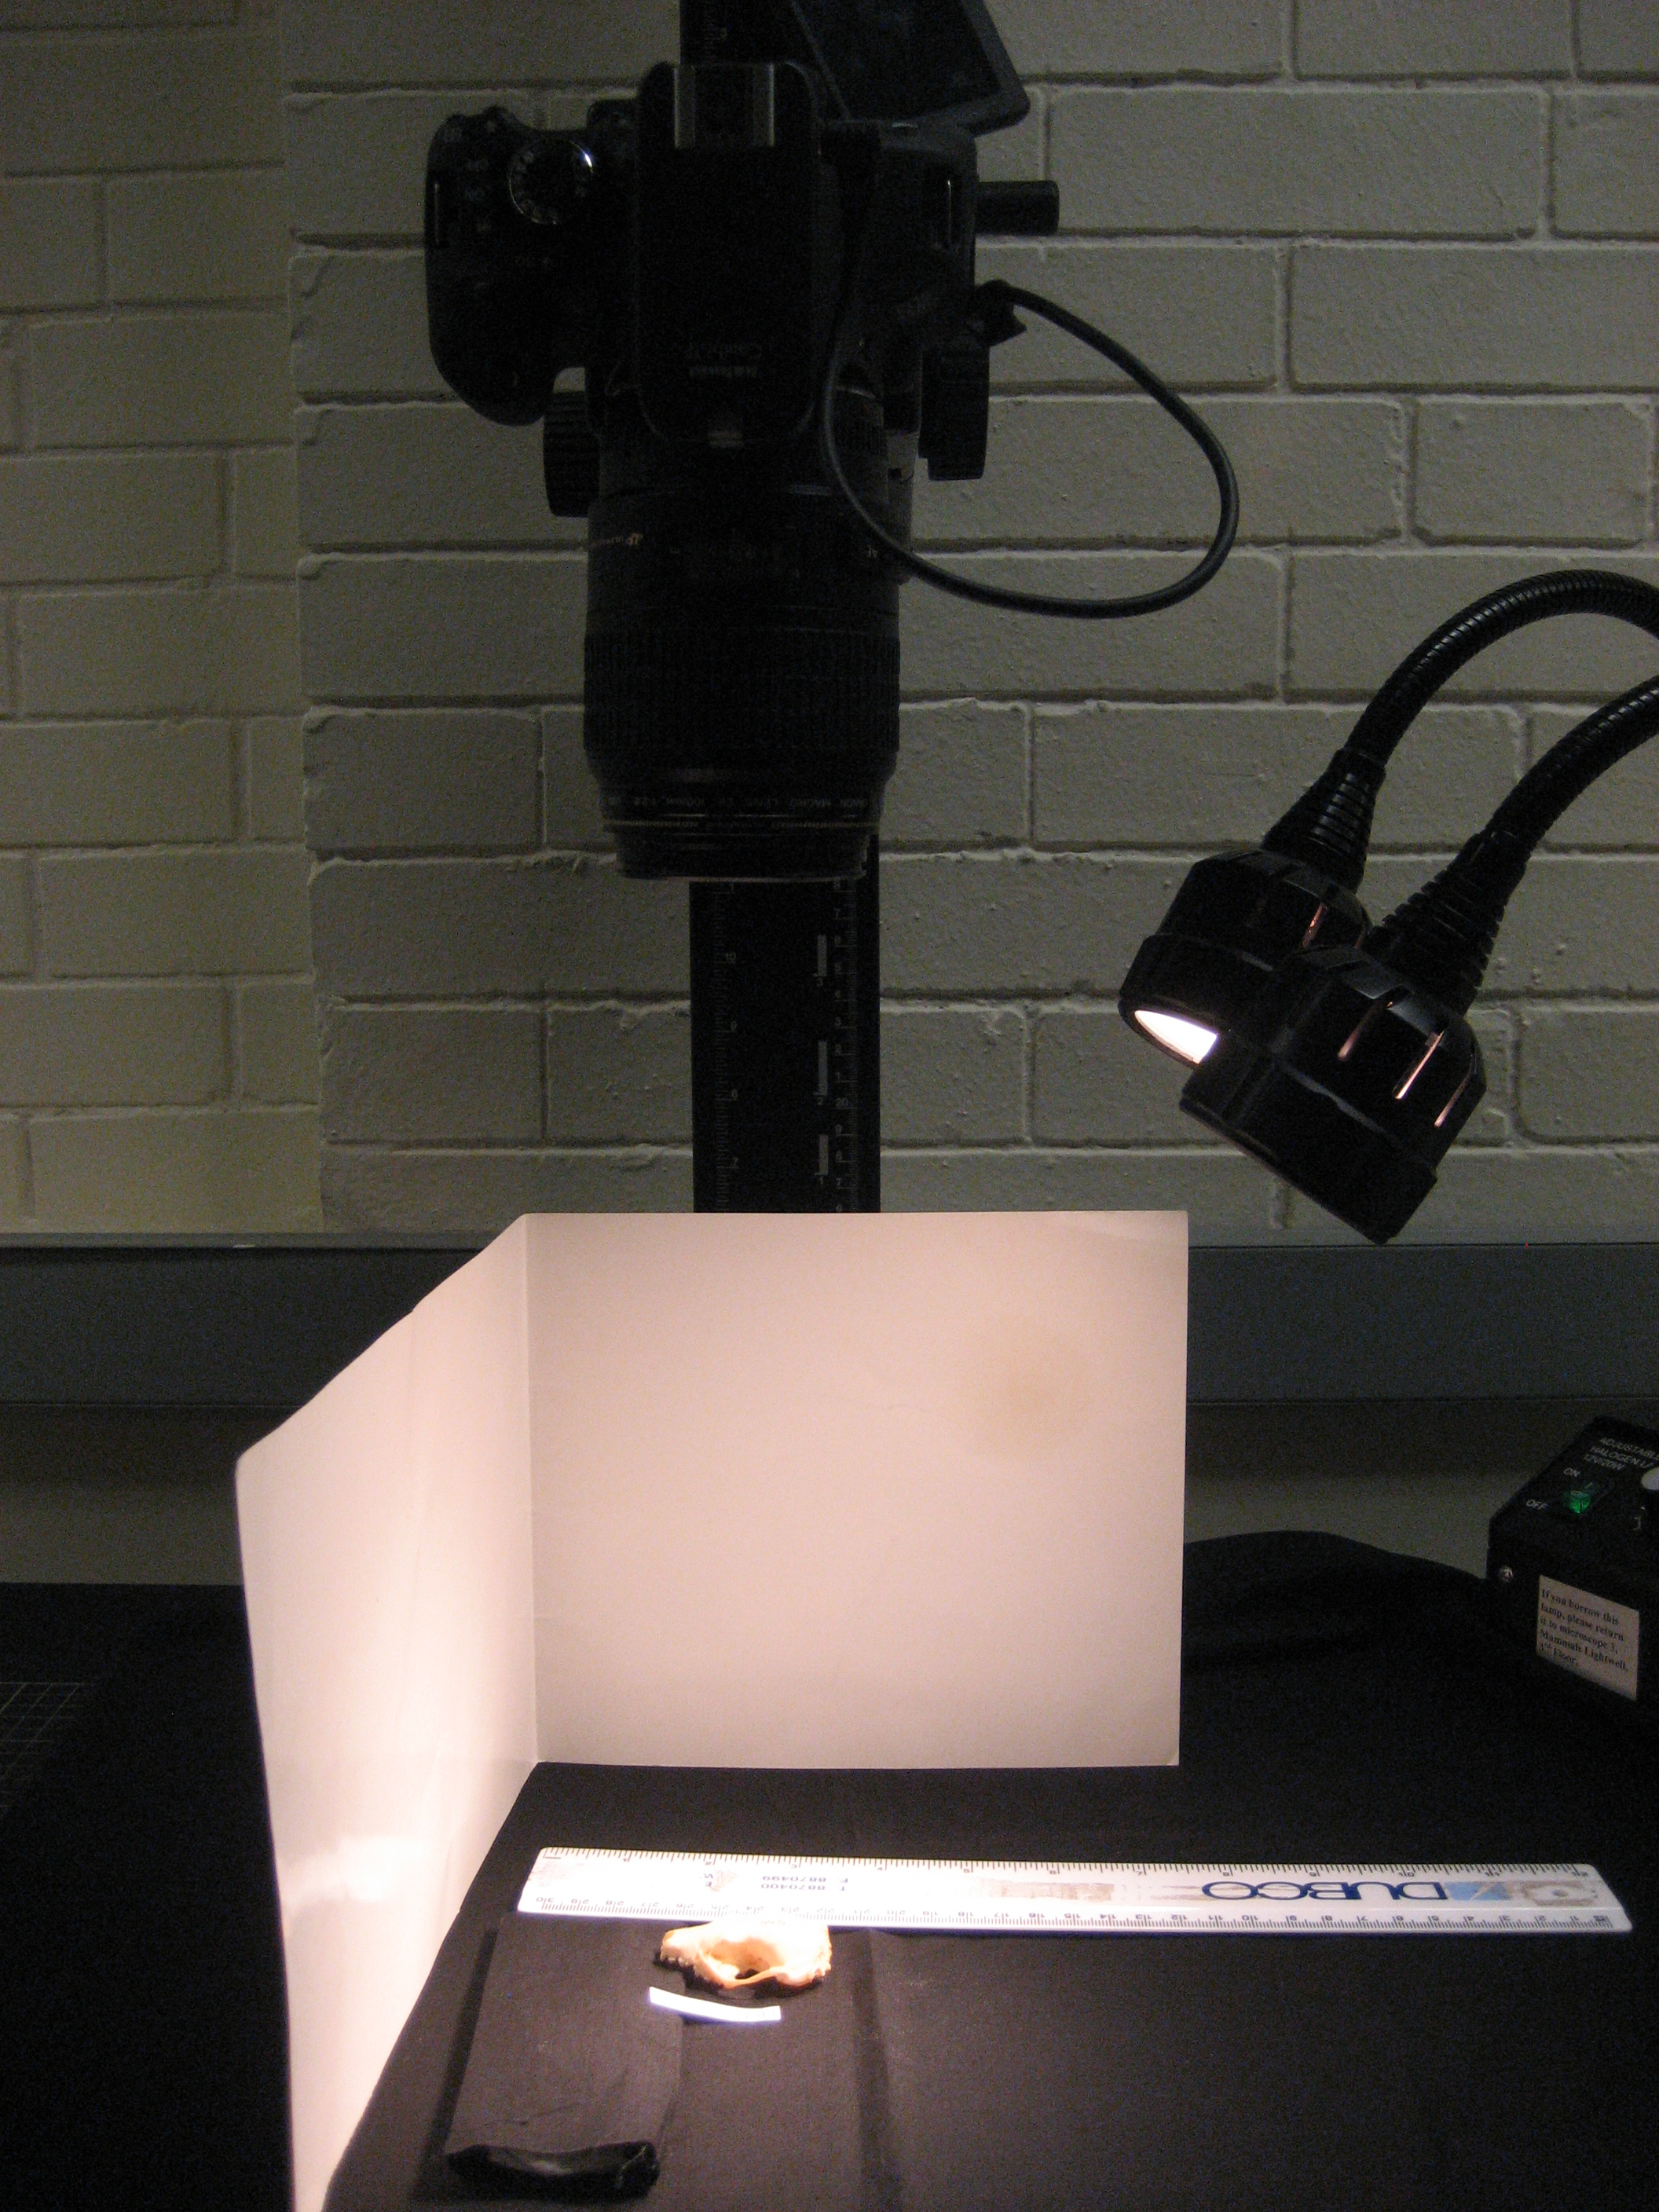
\includegraphics[width=12cm, height=12cm, keepaspectratio=true]{Methods/figures/camera.jpg}
    \caption[Photographic set up]
    {Photographic set up for taking pictures of skulls. The camera (above centre) is fitted to a copy stand, the light source is directed from the top-left corner of the image and the white card reflects the light back onto the skull. }
  \label{fig:camera}
  \end{figure}
%-------------------------------------------------

	I photographed the skulls in three views; dorsal (top of the cranium), ventral (underside of the skull with the palate roof facing uppermost) and lateral (right side of the skull). I also photographed the outer (buccal) side of the right mandible. When the right sides of either the skull or mandibles were damaged or incomplete I photographed the left sides and later reflected the images so that they could be compared to pictures of the right sides \citep[e.g.][]{Barrow2008}.


\subsection{\normalfont{Saving and processing images}}
	Photographs were captured and saved in a raw file format. Before using the photos for morphometric analyses, I converted the raw files to binary (grey scale) images and re-saved them as TIFF files. The black and white images were more useful for later analyses since I was not interested in including any colour comparisons and it is easier to see some biological features in binary images. TIFF files were also appropriate because they are uncompressed (in comparison to JPEG) images and therefore there is less chance of any picture distortions which may affect later analyses \citep{HERC2013}.
	Photographs of the specimens from the American Museum of Natural History and the Smithsonian Institute are available on figshare in separate file sets for the dorsal \citep{Finlay2013d}, ventral \citep{Finlay2013v} and lateral \citep{Finlay2013l} skull pictures along with the mandibles \citep{Finlay2013m}. Copyright restrictions from the other museums prevent public sharing of their images however they are available on request.
	

%##################################################

\section{Geometric morphometric analyses}
\label{sect:morphometrics}

\subsection{\normalfont{Landmark placement on images}}


	I used a combination of landmark and semilandmark analysis approaches to assess the shape variability in my skull and mandible specimens. 

	I used the TPS software suite \citep{Rohlf2013} to digitise landmarks and curves on the photos. I set the scale on each image individually to standardise for the different camera heights I used when photographing my specimens. I created separate data files for each of my four morphometric analyses (skulls in dorsal, ventral and lateral views and mandibles in lateral view). I digitised landmarks and semilandmark points on every image individually. Some specimens were too damaged to use so I had a different total number of images for each analysis: skulls dorsal (356), ventral (346), lateral (336) and mandibles (356).
	%Numbers are from the two_family_disparity script after cleaning up the data to remove damages specimens

	When combining landmark and semilandmark approaches, there is a potential problem of over-sampling the curves \citep{MacLeod2012}. To determine the number of semilandmark points required to adequately summarise the curves in my data sets I followed the method outlined by MacLeod \citeyearpar{MacLeod2012}. For each data set I chose a random selection of photos of specimens which represented the breadth of the morphological data (i.e. specimens from each sub-group of species). I drew the appropriate curves on each specimen and over-sampled the number of points on the curves. I measured the length of the line and regarded that as the 100\%, true length of that outline. I then re-sampled the curves with decreasing numbers of points and measured the length of the outlines. I calculated the length of each re-sampled curve as a percentage of the total length of the curve and then found the average percentage length for that reduced number of semilandmark points across all of the specimens in my test file. I continued this process until I found the minimum number of points that gave a curve length which was at least 95\% accurate.  I repeated these curve-sampling tests for each analysis to determine the minimum number of semilandmark points which would give accurate representations of morphological shape.
	
	Here I summarise the landmarks and curves which I used on each of my different sets of photos. For landmarks which are defined by dental structures, I used published dental sources \citep{Repenning1967, Eisenberg1969, Nowak1983, MacPhee1987, KnoxJones1992, Davis1997, Querouil2001, Nagorsen2002, Wilson2005, Goodman2006, Karatas2007, Hoffmann2008, Asher2008, Lin2010,  Muldoon2009} where available to identify the number and type of teeth in each species.
	
%------------------------------------------------------------------
\subsection{\normalfont{Skulls: dorsal view}}
	Most of my landmarks in this view are relative (type 3) points which represent overall morphological shape but not necessarily homologous biological features \citep{Zelditch2012}. I placed ten landmarks and drew four semilandmark curves to represent the shape of both the braincase (posterior) and nasal (anterior) area of the skulls (figure \ref{fig:skdors_skvent}). Table \ref{tab:skdors} describes how I placed the landmarks and drew the outline curves for my images of skulls in dorsal view.

\subsection{\normalfont{Skulls: ventral view}}

	Most of the landmarks in this view are concentrated around the dentition and palate of the animals. I placed 13 landmarks and drew one outline curve (resampled to 60 semilandmark points) around the back of the skull between landmarks 12 and 13 (figure \ref{fig:skdors_skvent}). The high variability of my species' basi-cranial region and difficulties associated with identifying developmentally or functionally homologous points precluded designation of additional landmarks towards the back of the skulls. Table \ref{tab:skvent} outlines the descriptions of the landmarks I placed on the ventral skull photos.

%------------------------------------------------
%Skulls dorsal and ventral

\begin{figure}[!htbp]
	\centering
	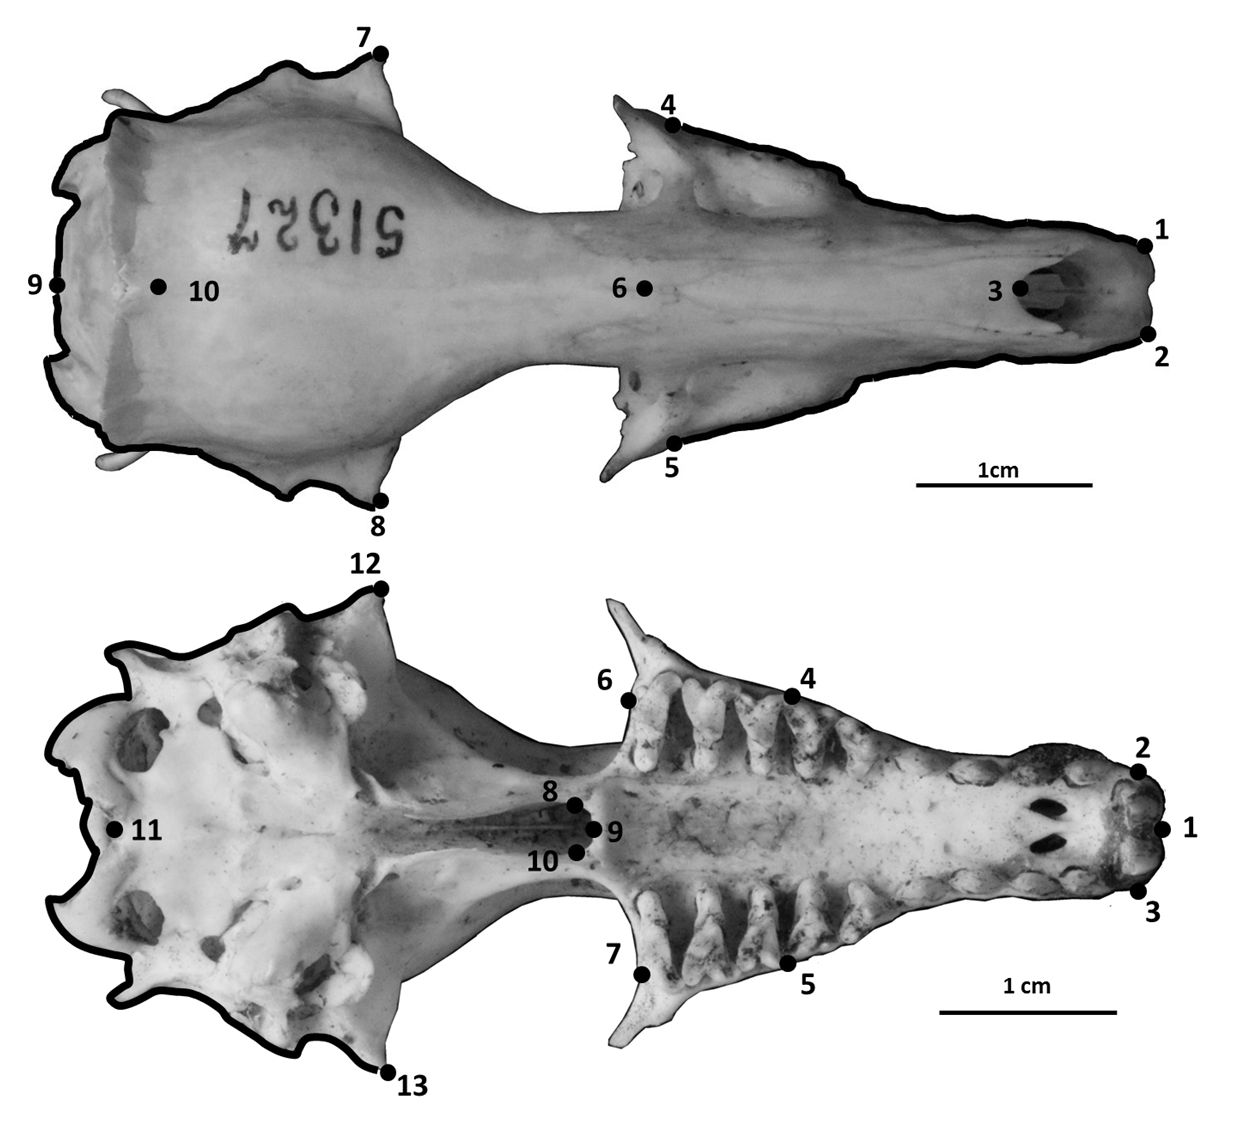
\includegraphics[width=1\linewidth]{Methods/figures/Skdors+Skvent_combined_BW.png}
	\caption[Skulls: dorsal and ventral landmarks]
	{Landmarks (numbered points) and curves(outlines) for the skulls in dorsal and ventral view. See tables \ref{tab:skdors} and \ref{tab:skvent} for landmark descriptions. The skulls are two different specimens of \textit{Potamogale velox} (otter shrew tenrec), museum accession numbers AMNH 51327 and BMNH 1934.6.16.2. }
	\label{fig:skdors_skvent}
\end{figure}


%Skdors descriptions
\begin{table}[h]
	\caption[Skulls: dorsal landmarks]
		{Descriptions of the landmarks (points) and curves (semilandmarks) for the skulls in dorsal view (figure
		\ref{fig:skdors_skvent})} 
	%Skdors landmarks

\begin{tabular}[t]{p{3cm}  l}		
\hline
\textbf{Landmark} & \textbf{Description} \\
\hline
%------------------------------------------------------------
1 + 2 & Left (1) and right (2) anterior points of the premaxilla \\
%------------------------------------------------------------
3 & Anterior of the nasal bones in the midline \\
%------------------------------------------------------------
4 + 5 &	Maximum width of the palate (maxillary) on the left (4) and right (5)\\
%------------------------------------------------------------
6 & Midline intersection between nasal and frontal bones \\
%------------------------------------------------------------
7 + 8 & Widest point of the skull on the left (7) and right (8) \\
%------------------------------------------------------------
9 &	Posterior of the skull in the midline \\
	%Panchetti 2008 and Macholan2008 have different definitions for this one so I need to choose one
%------------------------------------------------------------
10 & Posterior intersection between saggital and parietal sutures \\
%--------------------------------------
\hline
\textbf{Curve A} & Outline of the braincase on the left side, between landmarks 9 and 7\\ 
(12 points) & (does not include visible features from the lower (ventral) side of the skull) \\

\textbf{Curve B} & Outline of the palate on the left side, between landamarks 4 and 1 \\
(10 points) & (outline of the rostrum only, not the shape of the teeth)\\

\textbf{Curve C} &	Outline of the braincase on the right side, between landmarks 9 and 8 \\
(12 points) & (does not include visible features from the lower (ventral) side of the skull) \\

\textbf{Curve D} & Outline of the palate on the right side, between landamarks 5 and 2 \\
(10 points) & (outline of the rostrum only, not the shape of the teeth)\\
%------------------------------------------------------------
\hline
\end{tabular}
	\label{tab:skdors}
\end{table}

%Skvent descriptions
\begin{table}[!htb] %force the table to go up with the picture
\caption[Skulls: ventral landmarks]
		{Descriptions of the landmarks (points) and curves (semilandmarks) for the skulls in ventral view (figure \ref{fig:skdors_skvent}).} 
%SkVent landmarks
\begin{tabular}[t]{p{0.2\textwidth} p{0.75\textwidth}}		
\hline
\textbf{Landmark} & \textbf{Description} \\
\hline
%--------------------------------------
1 & Anterior point of the palate\\
%--------------------------------------
2 + 3 & Posterior, lateral extremity of the right (2) and left (3) incisor\\
%--------------------------------------
4 + 5 & Anterior, outer point of the first molar on the right (4) and left (5)\\
%--------------------------------------
6 + 7 & Posterior, outermost point of the last molar surface on the right (6) and left (7) \\
%--------------------------------------
8 & Widest point of the curve of the palatine on the right side\\
%--------------------------------------
9 & Posterior point of the palatine in the midline\\
%--------------------------------------
10 & Widest point of the curve of the palatine on the left side\\
%--------------------------------------
11 & Anterior of the occipital foramen in the midline\\
%--------------------------------------
12 + 13 & Widest (extreme lateral) point of the braincase on the right (12) and left (13)\\
%--------------------------------------
Curve*  & Outline of the back of the skull (between landmarks 12 and 13), 60 points \\
%------------------------------------------------------------
\hline
\end{tabular}
\label{tab:skvent}
\end{table}
%-------------------------------------------------------------

\subsection{\normalfont{Skulls: lateral view}}
	I placed nine landmarks on the photographs of skulls in lateral view (figure \ref{fig:sklat_mands}) and also drew two semilandmark curves to represent the shape of the back of the skull (between landmarks 7 and 8, resampled to 20 semilandmark points) and the top of the skull (between landmarks 8 and 1, resampled to 15 semilandmark points). Table \ref{tab:sklat} describes my definitions for each of the landmark points.
	If specimens were damaged on their right side I reflected photographs of the left lateral side of the skull so that all the images were in the same orientation.


\subsection{\normalfont{Mandibles}}
	I placed seven landmarks and drew four curves on each mandible photograph (again, reflecting any images of the left mandible so they were in the correct orientation, figure \ref{fig:sklat_mands}). I drew separate curves around each of the three processes of the ascending ramus: coronoid, condyloid and angular and along the base of the horizontal ramus of the jaw (figure \ref{fig:sklat_mands}, table \ref{tab:mands}). 	
%SF: Took out the paragraph about developmental independence in the jaw

%---------------------------------------------------
%Combined sklat and mandibles diagrams
\begin{figure}[!htbp]
	\centering
	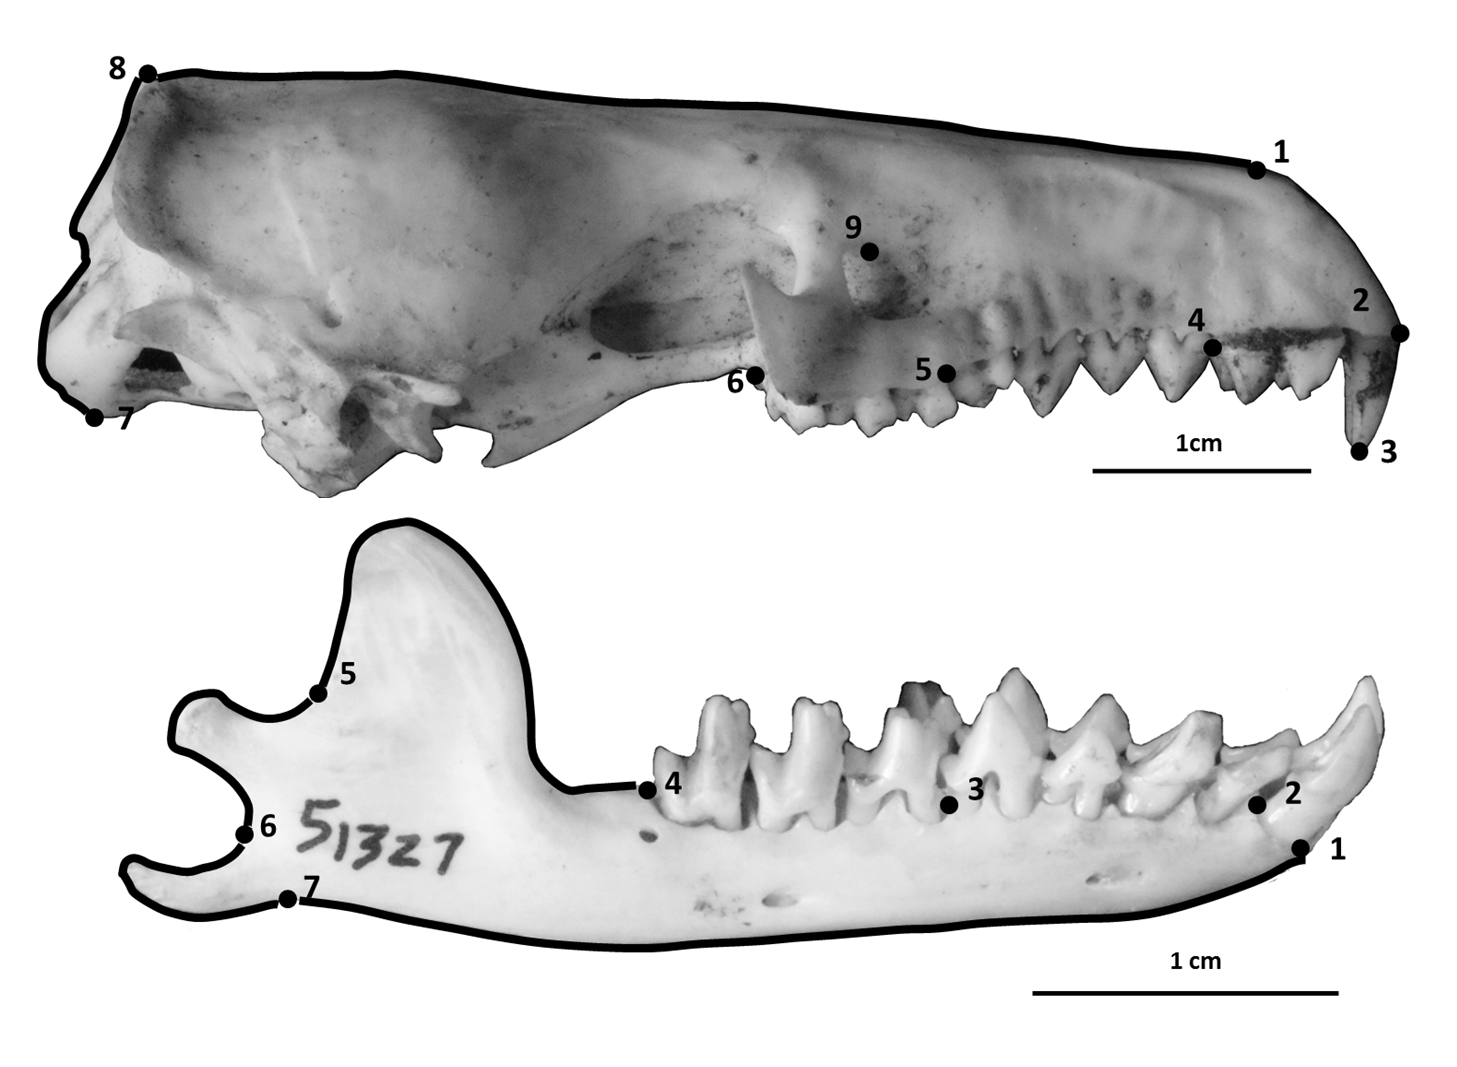
\includegraphics[width=1\linewidth]{Methods/figures/Sklat+mands_combined_BW.png}
	\caption[Lateral skulls and mandibles landmarks]
	{Landmarks (numbered points) and curves(outlines) for the skulls and mandibles in lateral view. See tables \ref{tab:sklat} and \ref{tab:mands} for landmark descriptions. The skull (BMNH 1934.6.16.2.) and mandible (AMNH 51327) belong to two different specimens of \textit{Potamogale velox} (otter shrew tenrec).}
	\label{fig:sklat_mands}
\end{figure}

%Sklat descriptions
\begin{table}[!htb]
\caption[Skulls: lateral landmarks]
		{Descriptions of the landmarks (points) and curves (semilandmarks) for the skulls in lateral view (figure \ref{fig:sklat_mands}).} 
%Sklat landmarks

\begin{tabular}[t]{p{2cm} p{12cm}}		
\hline
\textbf{Landmark} & \textbf{Description} \\
\hline
%--------------------------------------
1 & Anterior, upper tip of the nasal bone\\
%--------------------------------------
2 & Anterior of the alveolus of the first incisor\\
%--------------------------------------
3 & Lowest point of the first incisor\\
%--------------------------------------
4& Posterior of the alveolus of the last incisor \\
%--------------------------------------
5 & Anterior tip of the alveolus of the first molar\\
%--------------------------------------
6 & Posterior tip of the alveolus of the last molar\\
%--------------------------------------
7 & Lowest point of the basi-occipital (base of the back of the skull)\\
%--------------------------------------
8 & Highest point of the braincase\\
%--------------------------------------
9 & Highest point of the infraorbital foramen\\
%--------------------------------------
\hline
\textbf{Curve A} & Between points 7 and 8  \\
(20 points)& Back of the skull from the lowest to highest points\\
%------------------------------------------------------------
\textbf{Curve B} & Between points 8 and 1  \\
(15 points)&From the highest point of the braincase to the front of the nasal \\
%------------------------------------------------------------
\hline
\end{tabular}
\label{tab:sklat}
\end{table}

%Mandibles descriptions
\begin{table}[!htb]			
	\centering
	\caption[Mandibles: landmarks]
		{Descriptions of the landmarks (points) and curves (semilandmarks) for the mandibles in lateral (buccal) view (figure \ref{fig:sklat_mands}).}
	%Mandibles landmarks


\begin{tabular}[t]{p{0.2\textwidth} p{0.75\textwidth}}		
\hline
\textbf{Landmark} & \textbf{Description} \\
\hline
1 & Anterior of the alveolus of the first incisor \\
2 & Posterior of the alveolus of the first incisor \\
3 &	Anterior of the alveolus of the first molar \\
4 & Posterior of the alveolus of the last molar \\
5 & Maximum curvature between the coronoid and condylar processes\\
6 & Maximum curvature between the condylar and angular processes  \\
7 &	Maximum curvature between the angular process and the horizontal ramus \\
%---------------------------------------------------
\hline
Curve A & Condyloid process (between landmarks 4 and 5, 15 points)\\
Curve B & Condylar process (between landmarks 5 and 6, 15 points) \\
Curve C & Angular process (between landmarks 6 and 7, 15 points)  \\
Curve D & Base of the jaw (between landmarks 7 and 1, 12 points)  \\
%---------------------------------------------------
\hline
\end{tabular}
	\label{tab:mands} 
\end{table}
%------------------------------------


\newpage
\subsection{\normalfont{Procrustes superimposition}}
\label{sect:procrustes}

	After creating my files with the landmarks and semilandmarks placed on each photograph, I used TPSUtil \citep{Rohlf2012} to create "sliders" files that defined which points in the TPS files should be treated as semilandmarks \citep{Zelditch2012}. I conducted all further morphometric analyses in R version 3.0.2 \citep{Team2014} within the geomorph package \citep{Adams2013}.

	
	I used the gpagen function in the geomorph package \citep{Adams2013} to run a general Procrustes alignment \citep{Rohlf1993} of the landmark coordinates while sliding the semilandmarks by minimising Procrustes distance \citep{Bookstein1997}.
	I used these Procrustes-aligned coordinates of all specimens to calculate average shape values for each species which I then used for a principal components (PC) analysis with the plotTangentSpace function \citep{Adams2013}. 
	

%------------------------------------------------
\subsection{\normalfont{Potential morphometrics errors}}
	 
	While 2D methods are an accepted means of comparing morphological shape \citep[e.g.][]{Adams2004, Mitteroecker2009}, particularly for comparing skull morphologies of small mammals \citep[e.g.][]{Cardini2003, Panchetti2008, White2008, Barrow2008, Scalici2011}, the inherent discrepancies associated with comparing three dimensional objects using two dimensional pictures can introduce some potential problems of possible image distortion \citep{Arnqvist1998}. Similarly, human error with how landmarks are positioned on specimens could also introduce noise into further analyses. 
	
	In contrast to detailed intraspecific work \citep[e.g.][]{Bornholdt2008, Blagojevic2011} photographic or landmark placement errors are unlikely to be significant in my interspecific study since one would expect that the morphological variation among species is large enough to  be detected as a signal above any background noise associated with methodological error \citep{Arnqvist1998}. Nevertheless, it is still important to assess measurement error in a morphometric data set to increase confidence in the outcome of final analyses.
	I identified two possible sources of morphometric measurement error; specimen orientation and placement of landmarks.

	Variation in the orientation of specimens for photography is one of the main sources of error in 2D morphometric studies \citep{Adriaens2007}. If specimens are not placed on a flat plane or in a consistent position relative to the camera, areas of the object which are tilted towards the camera will appear to be larger than reality, distorting any subsequent morphometric analyses of the shape. 
	I placed the landmarks on each set of pictures so inter-observer variation in landmark placement is not an issue for my study.  However, repeatability and reliability of my choice of landmarks could affect the final results of my analyses \citep{Arnqvist1998}.
	%Need to fix this reference: it's okay in the bibliography but it doesn't all show up here

	To measure potential orientation error, I photographed the skulls (dorsal, ventral and lateral views) and mandibles of each specimen three times, cycling through the photos so that the specimen was removed and re-positioned before every shot \citep{Viscosi2011}.
	I used a subset of my ventral skull images to test for two sources of error: specimen orientation and landmark placement error \citep{Arnqvist1998, Barrow2008}. Of the specimens which I photographed three times,  I chose a random subset of seven skulls from four different Families: three tenrecs and single representatives of shrews, moles, hedgehogs and golden moles. I copied these images and placed landmarks on three copies of each image to compare variation in landmark placement within each orientation. This gave nine replicates of each skull: three separate photos, and three copies of each of those photos. As before, I ran a general Procrustes alignment \citep{Rohlf1993} of the specimens, calculated the average shape values for each skull (average of all nine pictures) and used these values for a principal components (PC) analysis. 
		
	I used a linear mixed effects model to model the shape variation (first PC axis) associated with specimen (fixed effect) and two nested random effects: photo identity nested within specimen and image replicate nested within each photograph. This nested approach was necessary to deal with the hierarchical nature of my data subset: three photos of every specimen and three replicates of each of those images. I ran the test using the lmer function in the lme4 package \citep{Bates2014}.  

	I found that specimen orientation and landmark placement have negligible effects on the overall shape variation between different skulls: the random effect variables of photo identify and image replicate explained less than 0.0001 \% of the overall shape variation among different skulls. Therefore, I am confident that shape variation between the specimens in the rest of my analyses reflected true morphological differences rather than methodological error.







